%!TEX root = ../main.tex

\begin{refsection}

\section{Basics of fault tolerance}\label{prim:FaultTolerance}

\subsubsection*{Rough overview (in words)}

The error rates of all known realizations of physical qubits and basic operations are too high to enable implementation of the majority of quantum algorithms considered in this survey.
Even if the probability $p$ for each basic operation to malfunction was minute, we would nevertheless expect an error to occur in any quantum circuit comprising more than $\bigO{1/p}$ operations.
One may optimistically assume that in the foreseeable future $p= 10^{-6}$ might be achieved by certain quantum architectures, such as trapped ions~\cite{bermudez2017trappedIonFaultTolerant,bruzewicz2019trappedIonProgressChallenges}.
This, in turn, limits the size of any quantum circuit that one may hope to reliably execute to roughly one million basic operations.  
Such a bound places a severe restriction on the algorithms that could be run and is orders of magnitude smaller than the resources needed to implement the quantum algorithms described in the other parts of this survey. 


The theory of quantum fault tolerance~\cite{shor1996FTQC} and quantum error correction~\cite{shor1995SchemeReducingDecoherence,steane1996ErrorCorrectingQuantum,gottesman1996QECCodesSaturatingHammingBound} provides a collection of techniques to deal with imperfect operations and unavoidable noise afflicting the physical hardware, at the expense of moderately increased resource overheads.
In the basic model for fault tolerance one assumes that each elementary component of a quantum circuit (including the identity gate) may fail with some small but nonzero probability, independently of the other components, and classical information processing is noiseless.
For concreteness and simplicity, one may choose to model any noisy component as an ideal component followed by (or, in the case of measurements, preceded by) some Pauli channel acting on the same subset of qubits.
Let $\mathcal C$ be a quantum circuit (possibly with classical input and output) describing a desired quantum algorithm.
Since each component of $\mathcal C$ may fail, one should not implement $\mathcal C$ directly; rather, one needs to implement a different quantum circuit $\mathcal F(\mathcal C)$, which is fault-tolerant (FT) version of $\mathcal C$.
This, in turn, can be achieved by replacing each qubit in $\mathcal C$ with a logical qubit encoded in some quantum error-correcting (QEC) code and each elementary component of $\mathcal C$ with a corresponding FT gadget; see Fig.~\ref{fig:FTcircuits}.
The desired quantum computation will then be realized on the logical level of $\mathcal F(\mathcal C)$ without leaving the protective encoding guaranteed by the QEC code.

\begin{figure}[h]
\centering
\begin{displaymath}
(a)\quad\quad\ \ \Qcircuit @C=.7em @R=.3em {
\lstick{\ket{+}} 	& \ctrl{1}	& \qw	& \gate{M_Z} \\
\lstick{\ket{0}}	& \targ	& \ctrl{1} 	& \gate{M_X} \\
\lstick{\ket{+}} 	& \gate{T}	& \targ	& \gate{M_X} 
}
\quad\quad\quad
(b)\quad\quad\ \ 
\Qcircuit @C=.7em @R=.3em {
\lstick{\ket{\overline +}}&\gate{\rm{QEC}}&\multigate{1}{\overline{CX}}&\gate{\rm{QEC}}& \gate{\overline I}			&\gate{\rm{QEC}}& \gate{\overline{M_Z}} \\
\lstick{\ket{\overline 0}}&\gate{\rm{QEC}}&\ghost{\overline{CX}}		&\gate{\rm{QEC}}&\multigate{1}{\overline{CX}}	&\gate{\rm{QEC}}& \gate{\overline{M_X}} \\
\lstick{\ket{\overline +}}&\gate{\rm{QEC}}&\gate{\overline T}		&\gate{\rm{QEC}}&\ghost{\overline{CX}}		&\gate{\rm{QEC}}& \gate{\overline{M_X}} 
}
\end{displaymath} 
\caption{(a) A quantum circuit $\mathcal C$ consists of state preparation, unitary gates, and measurements.
(b) An FT realization of $\mathcal C$ is a quantum circuit $\mathcal F(\mathcal C)$ obtained by replacing each qubit in $\mathcal C$ with a logical qubit encoded in some QEC code and using appropriate FT gadgets interspersed with QEC gadgets in place of each basic component of $\mathcal C$.
Note that some gadgets may require considerable resources (not shown in the picture); see \hyperref[prim:LatticeSurgery]{logical gates} and \hyperref[prim:QEC]{QEC gadgets} with the surface code for more details.
}
\label{fig:FTcircuits}
\end{figure}


To realize universal FT quantum computation, it suffices to have state preparation gadgets (for at least one type of state), measurement gadgets (for at least one type of measurement), gate gadgets (for a universal set of gates) and QEC gadgets.
One requires that all these gadgets satisfy certain FT conditions; see, for instance, \cite{aliferis2006quantum,gottesman2010introduction}.
Although the asymptotic scaling of resource overheads associated with FT gadgets is manageable (for instance, polylogarithmic in the inverse of the target logical error rate), the constant prefactors tend to be large, resulting in the qubit and time overheads
that currently constitute one of the main bottlenecks to practical FT quantum computation.
We will discuss this point in more detail for the implementation of \hyperref[prim:LatticeSurgery]{logical gates} and \hyperref[prim:QEC]{QEC gadgets}
with the planar architecture based on the surface code~\cite{kitaev1997FTQCanyons,dennis2002TopologicalQuantumMemory}.

%%%%%%%%%%%%%%%%%%%%%%%%%%%%%%%%%%%%%%%%%%%%%%%%%%%%%%%%%%%%%%%%%%%%%%

\subsubsection*{Rough overview (in math)}

Designing FT gadgets is a challenging task for several reasons.
First, FT gadgets are usually developed and optimized for a specific QEC code.
Second, even though they comprise imperfect basic components, they are required to work reliably as long as a number of malfunctioning components is limited.
Third, FT gadgets may spread errors, however they must not do so in an uncontrollable way.  

Given a set of FT gadgets, one can reliably perform an arbitrarily long quantum computation as long as the physical error rate of each basic component is below some constant value, often referred to as the FT threshold.
This result is established by the celebrated threshold theorem~\cite{aharonov1997FTQCconstantError,kitaev1997quantumComputationsAlgosQEC,knill1998ResilientQC,aliferis2006quantum}.
To be more precise, consider the basic model for FT.
The threshold theorem asserts that there exists a constant $p_\text{FT}>0$, such that for any $\epsilon>0$ and any quantum circuit $\mathcal C$ there exists a quantum circuit $\widetilde{\mathcal C}$ that produces an output with statistical distance at most $\epsilon$ from the output of $\mathcal C$, provided the physical error rate $p$ is below $p_\text{FT}$.
Moreover, $\widetilde{\mathcal C}$ uses a number of qubits and timesteps that are at most $\mathrm{polylog}(|\mathcal C|/\epsilon)$ times bigger than the number of qubits and timesteps in $\mathcal C$, where $|\mathcal C|$ denotes the number of basic components in $\mathcal C$.


The basic idea behind the proof of the threshold theorem proceeds as follows.
Consider a quantum circuit $\mathcal F(\mathcal C)$, which is an FT implementation of $\mathcal C$. 
Assuming the basic model for fault tolerance described above, for sufficiently small physical error rate $p$, the logical error rate for $\mathcal F(\mathcal C)$ should be smaller than $p$, since $\mathcal F(\mathcal C)$ is an FT implementation of $\mathcal C$.
One can then consider a quantum circuit $\mathcal F\circ \mathcal F(\mathcal C)$, which is an FT implementation of $\mathcal F(\mathcal C)$, reducing the logical error rate even further.
By repeating this process, one eventually obtains a quantum circuit $\widetilde{\mathcal C} = \mathcal F\circ\ldots \circ \mathcal F(\mathcal C)$ with the logical error rate below $\epsilon$.
The resulting FT protocol is based on concatenated QEC codes.


One may improve the scaling of the resource overheads from the threshold theorem with concatenated QEC codes.
In particular, in the asymptotic limit of large quantum circuits, the ratio of qubits in $\mathcal C$ and $\widetilde{\mathcal C}$ can be a constant~\cite{gottesman2014FTQCconstantOverhead}.
In this construction, the FT protocol requires a family of QEC codes that satisfies certain properties, including the desired scaling of code parameters, computationally efficient decoding algorithms and constant-weight parity checks.
Such a family of QEC codes was first provided in~\cite{fawzi2018ConstantOverheadExpanderCode}.

%%%%%%%%%%%%%%%%%%%%%%%%%%%%%%%%%%%%%%%%%%%%%%%%%%%%%%%%%%%%%%%%%%%%%%

\subsubsection*{Dominant resource cost (gates/qubits)}

At the heart of FT quantum computation, there is usually some QEC code.
Since the choice of a QEC code affects the resource overheads, we would like to choose one for which the encoding rate (defined as the ratio $k/n$, where $k$ and $n$ are the number of logical and physical qubits, respectively) as well as the relative code distance (defined as the ratio $d/n$, where $d$ is the minimum weight of any nontrivial logical operator) are as high as possible.
Although for concatenated QEC codes (that feature in the threshold theorem), both $k/n$ and $d/n$ go to zero as $n$ goes to infinity, we know that there exist QEC codes with good parameters, i.e, for which $k/n$ and $d/n$ are asymptotically constant~\cite{calderbank1996GoodQECCodes}.
Moreover, recent groundbreaking results~\cite{breuckmann2021balancedProductQuantumCodes,panteleev2022GoodLDPC,dinur2022LocallyTestable,leverrier2022QuantumTannerCodes} provided constructions of QEC codes that not only have good parameters but also constant-weight parity checks (thus their name---quantum low-density parity check codes).
The latter property is particularly important from the perspective of fault tolerance.
However, experimental realization of these constructions (in contrast to \hyperref[prim:QEC]{the surface code}) seems extremely challenging, at least within the realm of solid-state qubits constrained by geometric locality of their physical entangling gates. 


Another aspect of FT quantum computation that affects the resource overheads are the FT gadgets that are being used.
One of the easiest ways to implement FT gadgets for gates is via transversal gates.
By definition, transversal gates are implemented via a tensor product of single-qubit unitaries (or, more generally, via a depth-one quantum circuit) and therefore do not spread errors in an uncontrollable way.
Unfortunately, transversal gates are limited by the Eastin--Knill theorem~\cite{eastin2009RestrictionsTransversal,zeng2011Transversality,jochymOConnor2018Disjointness,kubica2021QuantumMetrologicalBounds}, which rules out the existence of a (finite-dimensional) QEC code with a universal set of transversal logical gates.
One strategy to circumvent this limitation is to prepare certain magic states and use them to realize FT gates~\cite{bravyi2005UniversalQC}; see the section on \hyperref[prim:LatticeSurgery]{implementing logical gates} for more details and a discussion of other strategies.


To realize FT gadgets for state preparation, QEC, and measurement, one typically chooses among three standard FT schemes: Shor's~\cite{shor1996FTQC}, Steane's~\cite{steane1997ActiveStabilization}, or Knill's~\cite{knill2005QCwithNoisyDevices}.
Roughly speaking, Shor's scheme uses simple states (verified cat states) of the ancilla qubits at the expense of implementing many gates on the data qubits, whereas Steane's and Knill's schemes trade highly complex states of the ancilla qubits (logical states encoded in the underlying QEC code) for minimizing the number of gates on the data qubits. 
To determine the best choice, one needs to consider the underlying QEC code (e.g., Steane's scheme is applicable only to CSS codes~\cite{calderbank1996GoodQECCodes,steane1996ErrorCorrectingQuantum}) and the quantum hardware restrictions (e.g., lack of extra ancilla qubits).
For an illuminating and detailed discussion of FT schemes, see, e.g.,  \cite{gottesman2010introduction}.
We remark that for QEC codes with additional structure, such as quantum low-density parity check codes, one may pursue different approaches toward FT quantum computation; see the section on \hyperref[prim:QEC]{QEC with the surface code}.


%%%%%%%%%%%%%%%%%%%%%%%%%%%%%%%%%%%%%%%%%%%%%%%%%%%%%%%%%%%%%%%%%%%%%%

\subsubsection*{Caveats}

Rigorous proofs provide lower bounds on the FT threshold $p_\text{FT}$.
For instance, for an FT scheme based on the $7$-qubit code, one finds $p_\text{FT} > 2.73\times 10^{-5}$ \cite{aliferis2006quantum}.
For an FT scheme by Knill~\cite{knill2005QCwithNoisyDevices} that relies on complex ancilla preparation techniques, one finds $p_\text{FT} > 1.04\times 10^{-3}$ \cite{aliferis2008AccuracyThresholdPostselected}.
However, these values can differ by orders of magnitude from the values estimated in numerical simulations.
For instance, the FT scheme by Knill is estimated to have an FT threshold $p_\text{FT}$ as high as $5\times 10^{-2}$, constituting one of the highest known FT thresholds. 
We remark that these values depend sensitively on the details of the FT schemes and the assumptions about noise.
In particular, to obtain the aforementioned values we assume the ability to implement gates between any qubits.
On the other hand, if we arrange qubits on some geometric lattice and restrict gates to be local, then FT thresholds still exist, however their values are significantly reduced.

One can expand the threshold theorem in many ways.
Even using the basic model for fault tolerance, one may choose the failure probabilities for each elementary component of a quantum circuit differently, e.g., the failure probability of a measurement to be ten times higher than that of a gate. 
One can consider more general noise (which includes systematic errors, such as overrotations) arising due to a weak interaction between the system and a non-Markovian environment~\cite{aliferis2006quantum,terhal2005FTQCnonMarkovian}.
In general, although experimental realizations of quantum computation may not satisfy exactly the assumptions of the threshold theorem, we expect the main conclusions to hold as long as the assumptions are not violated too much.

To simplify the analysis of FT schemes, we often assume unlimited classical computational power that one needs to, e.g., process the error syndrome and infer an appropriate recovery operator in a QEC gadget; a number of such decoding algorithms have been developed for \hyperref[prim:QEC]{QEC with the surface code}.
It is important not to abuse this assumption by, for instance, solving the initial problem with an inefficient classical algorithm.
At some point, however, one needs to take into account the finite speed of classical information processing.
If the classical unit that processes the error syndrome is unable to keep pace with the rate at which this syndrome is being produced, then the error syndrome will start to accumulate and one will suffer from the so-called backlog problem~\cite{terhal2015QECforQuantumMemories}. 
Subsequently, the speed of quantum computing will be exponentially reduced and the computational advantage of quantum computing will be annulled.
This issue will be especially prominent for polynomial speedup quantum algorithms.



%%%%%%%%%%%%%%%%%%%%%%%%%%%%%%%%%%%%%%%%%%%%%%%%%%%%%%%%%%%%%%%%%%%%%%

\subsubsection*{Further reading}
\begin{itemize}
    \item An accessible introduction to quantum error correction and the theory of fault tolerance can be found in  \cite{raussendorf2012KeyIdeasQEC}.
    \item A detailed introduction to quantum error correction and fault-tolerant quantum computation can be found in  \cite{gottesman2010introduction}.
    \item A fairly recent perspective on roads towards fault-tolerant universal quantum computation can be found in  \cite{campbell2017RoadsTowardFTQC}.
    \item The \href{https://errorcorrectionzoo.org/}{error correction zoo} provides a useful compilation of error correcting codes.
\end{itemize}

%%%%%%%%%%%%%%%%%%%%%%%%%%%%%%%%%%%%%%%%%%%%%%%%%%%%%%%%%%%%%%%%%%%%%%
\printbibliography[heading=secbib,segment=\therefsegment]

\end{refsection}



\newpage


%%%%%%%%%%%%%%%%%%%%%%%%%%%%%%%%%%%%%%%%%
%%%%%%%%%%%%%%%%%%%%%%%%%%%%%%%%%%%%%%%%%

\begin{refsection}
\section{Quantum error correction with the surface code}
\label{prim:QEC}

\subsubsection*{Rough overview (in words)}


To protect quantum information from detrimental effects of noise, we can encode it into a code space of some quantum error correcting (QEC) code~\cite{shor1995SchemeReducingDecoherence,steane1996ErrorCorrectingQuantum}.
Oftentimes, we choose to work with stabilizer codes~\cite{gottesman1996QECCodesSaturatingHammingBound}.
By definition, a code space of a stabilizer code is the simultaneous $(+1)$-eigenspace of a set of commuting Pauli operators, commonly referred to as parity checks.


The surface code~\cite{kitaev1997FTQCanyons,bravyi1998quantumCodesLattice,dennis2002TopologicalQuantumMemory} is one of the most-studied stabilizer codes.
It can be implemented with a planar layout of qubits and entangling gates only between neighboring qubits.
For that reason, the surface code is particularly appealing for quantum hardware architectures with restricted qubit layout and connectivity, such as superconducting circuits~\cite{devoret2013superconductingCircuits,blais2021circuitQuantumElectrodynamics}.
The most common realization of the surface code uses $n = L^2$ data qubits to encode $k=1$ logical qubit and has code distance $d=L$, where $L$ is the linear size of the $L\times L$ square lattice with open boundary conditions.
Additionally, $n_A = L^2 -1$ ancilla qubits are used to measure parity checks; see \cref{fig:surface_code}(a).


\begin{figure}[h]
\centering
(a)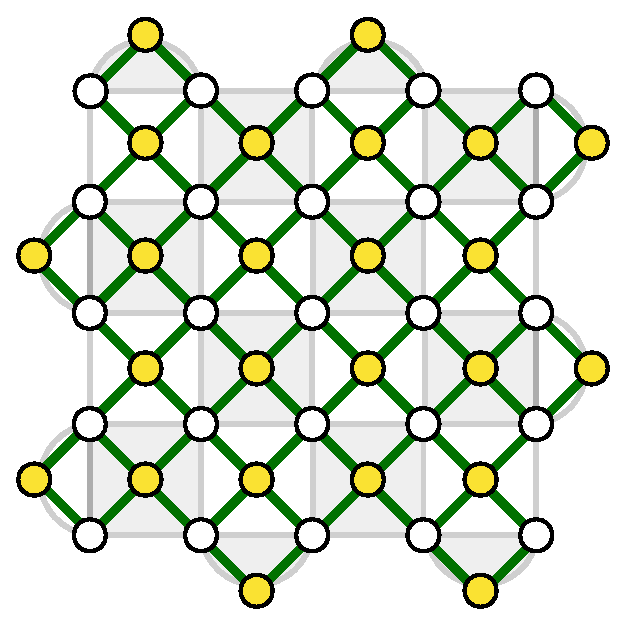
\includegraphics[draft=false,height=0.171\textheight]{figures/fig_surface_layout}\quad\quad\quad
(b)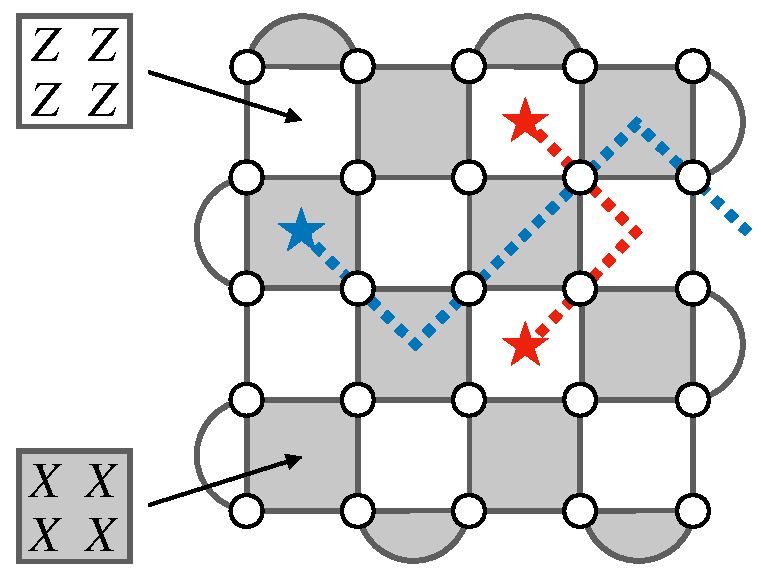
\includegraphics[draft=false,height=0.165\textheight]{figures/fig_surface_error_same}
\caption{
(a) A planar layout of data and ancilla qubits (white and yellow dots, respectively) with entangling gates (green edges) only between neighboring qubits.
This layout gives rise to the $L\times L$ square lattice with open boundary conditions, where $L=5$ here.
(b) The surface code can be realized by measuring Pauli $Z$- and $X$-type parity checks (light and dark faces, respectively). 
The error syndrome (red and blue stars) can be interpreted as the endpoints of string-like Pauli $X$ and $Z$ errors (red and blue dashed edges, respectively).
}
\label{fig:surface_code}
\end{figure}


In order to perform QEC, we have to be able to detect errors without revealing the encoded information.
For stabilizer codes, we can achieve that by measuring their parity checks to obtain the error syndrome (which comprises the measurement outcomes returning $-1$).
Then, the error syndrome is processed by specialized classical algorithms, also known as ``decoders,'' to find an appropriate recovery operator that attempts to remove errors afflicting the encoded information.
For generic stabilizer codes, the problem of optimal decoding is computationally hard, even for simple noise models~\cite{iyer2015hardnessDecoding}.
However, for QEC codes with some underlying structure, such as the surface code, there exist a variety of computationally efficient (albeit not optimal) decoding algorithms.
In particular, the three most popular classes of decoders for the surface code are as follows.
\begin{itemize}
\item Matching decoders, including the minimum-weight perfect matching algorithm~\cite{dennis2002TopologicalQuantumMemory} and its follow-up improvements, such as the belief-matching algorithm~\cite{higgott2023improvedDecodingCircuitNoise}.
These decoders phrase the problem of surface code decoding as a graph-theoretic problem of perfect matching, which can be efficiently solved~\cite{edmonds1965pathsTreesFlowers}.
\item Clustering decoders, such as the renormalization-group decoder~\cite{duclosCianci2010fastDecoders,anwar2014fastDecoders} and the union-find decoder~\cite{delfosse2021almostLinearTimeDecoding}.
These decoders primarily exploit the structure of the error syndrome in the surface code; see Fig.~\ref{fig:surface_code}(b).
\item Tensor-network decoders~\cite{bravyi2014efficientAlgorithmsMaxLikelihood,darmawan2017tensorNetworkSurfaceCode,chubb2021tensorNetworkDecoding}.
These decoders phrase the the problem of surface code decoding as a numerical problem of contracting tensor networks.
\end{itemize}


In order to assess the usefulness of decoders, one usually considers two criteria: runtime and performance.
The first criterion, runtime, is defined as the time needed for the decoder to process the error syndrome.
It is crucial that any practical decoder is able to operate at the rate compatible with the rate of parity check measurements; otherwise, the error syndrome will start to accumulate, leading to the backlog problem~\cite{terhal2015QECforQuantumMemories}.
The second criterion, performance, is typically defined for a given noise model in terms of the logical error rate, i.e., the failure rate of the decoder to successfully undo the effects of noise on the encoded information.
From the perspective of reducing runtime and improving performance, matching and clustering decoders stand out.
Namely, they can achieve almost-linear runtime~\cite{higgott2023sparseBlossom,delfosse2021almostLinearTimeDecoding}, and their performance is close to optimal.
To achieve optimal performance, one can use tensor-network decoders, however they are often not computationally efficient, with runtime that scales unfavorably.


%%%%%%%%%%%%%%%%%%%%%%%%%%%%%%%%%%%%%%%%%%%%%%%%%%%%%%%%%%%%%%%%%%%%%%

\subsubsection*{Rough overview (in math)}


In addition to being compatible with planar layouts of qubits and admitting computationally efficient decoders with good performance, the surface code also exhibits one of the highest QEC thresholds.
Recall that a QEC threshold is specified for the following triple: a QEC code family of growing distance $d$, a decoder and noise model.
It is defined as the highest value $p_\text{th}$ such that for any error rate $p< p_\text{th}$ the probability that the decoder fails to undo the effects of noise goes to zero as $d$ goes to infinity. 
For example, the QEC threshold for the surface code, using minimum-weight perfect matching algorithm, with a circuit noise model based on depolarizing noise, is around $1\%$~\cite{wang2011surfaceCodeErrorRates,higgott2023improvedDecodingCircuitNoise}.


Typically, if the error rate $p$ describing noise is sufficiently low and below the threshold $p_\mathrm{th}$, then the logical error rate $p_\mathrm{fail}$ scales as follows
\begin{equation}
p_\mathrm{fail} \sim \left(\frac{p}{p_\mathrm{th}}\right)^{\left\lceil \frac{d}{2}\right\rceil}.
\end{equation}
This implies that in order to achieve the target error rate $\epsilon$, it suffices to implement the surface code with code distance
$d = \bigO{\log(1/\epsilon) / \log(p_\text{th}/p)}$ using $n + n_A = \bigO{d^2} = \bigO{\log^2(1/\epsilon) / \log^2(p_\text{th}/p)}$ data and ancilla qubits.
Subsequently, qubit overhead associated with QEC based on the surface code only scales polylogarithmically in the inverse target error rate $1/\epsilon$.


%%%%%%%%%%%%%%%%%%%%%%%%%%%%%%%%%%%%%%%%%%%%%%%%%%%%%%%%%%%%%%%%%%%%%%

\subsubsection*{Dominant resource cost (gates/qubits)}


Performing reliable QEC in the presence of measurement errors becomes challenging since the error syndrome can be corrupted.
A straightforward solution to the problem of unreliable error syndrome is to repeatedly measure the parity checks in order to gain enough confidence in their measurement outcomes~\cite{shor1996FTQC,dennis2002TopologicalQuantumMemory}.
If this approach is applied to the surface code with code distance $d$, then one needs to perform $\bigO{d}$ rounds of parity check measurements, incurring relatively large time overhead.


To reduce time overhead, one can pursue single-shot QEC~\cite{bombin2015SingleShotFTQEC}, which does not require repeated measurement rounds.
It is possible to realize single-shot QEC with the surface code~\cite{campbell2019theorySingleShot, ashikhmin2020quantumDataSyndromeCodes, delfosse2022beyondSingleShotFTQC}, however, in addition to parity checks in~\cref{fig:surface_code}(b), one would need to measure nonlocal high-weight parity checks, which is a serious limitation.
A more streamlined approach is to consider a different realization of the surface code, the three-dimensional subsystem toric code~\cite{kubica2022singleShotQECtoric,bridgeman2023liftingTopologicalCodes}, which can be implemented with qubits arranged on the cubic lattice and local low-weight parity checks.
Although this approach is natively defined in three spatial dimensions, it can be emulated with planar layouts of qubits and either a limited number of nonlocal gates or the ability to reshuffle qubits (which is available with, e.g., Rydberg atoms~\cite{saffman2010quantumInfoRydberg,browaeys2020manyBodyRydberg}).
In order to realize code distance $d$ one incurs qubit overhead of $\bigO{d^3}$ (compared to qubit overhead of $\bigO{d^2}$ for the surface code).
From that perspective, single-shot QEC with the subsystem toric code can be viewed as trading time overhead for qubit overhead.


%%%%%%%%%%%%%%%%%%%%%%%%%%%%%%%%%%%%%%%%%%%%%%%%%%%%%%%%%%%%%%%%%%%%%%

\subsubsection*{Caveats}

There have been efforts to improve surface code decoders by incorporating various machine learning methods, including neural networks~\cite{torlai2017neuralDecoder,maskara2019advantagesNeuralNetworkDecoding,chamberland2022techniquesLocalGlobalDecoders} and reinforcement learning~\cite{sweke2021reinforcementLearningDecoders}.
At the current stage, decoders solely based on machine learning methods seem to be of limited applicability, mostly due to high training costs and scalability issues.
Nevertheless, these approaches are likely to be immensely beneficial for QEC in the settings where (possibly correlated) noise is unknown and may have to be learned first. 


Typically, in QEC analysis one considers simple Pauli noise, such as depolarizing noise acting independently and identically on each qubit.
If noise exhibits bias between the $X$, $Y$, and $Z$ components of Pauli noise, then this structure can be exploited, leading to dramatically increased QEC thresholds, as exemplified by variants of the surface code~\cite{tuckett2018ultrahighErrorThreshold,bonillaAtaides2021XZZXsurfaceCode,dua2022cliffordDeformed}.
Similarly, noise that is biased toward erasure errors can be beneficial from the perspective of QEC~\cite{stace2009thresholdsTopologicalCodes,wu2022erasureConversion,kubica2022erasure}.
On the other hand, realistic noise may be coherent or correlated and thus not only difficult to correct, but also to numerically simulate.
For instance, the logical error rates for coherent noise may be orders of magnitude higher than the estimates of the logical error rates for simple Pauli noise (assuming both types of noise have the same error rate)~\cite{iyer2018smallQCneeded}.


In addition to the three-dimensional subsystem toric code, one can also consider other higher-dimensional versions of the surface code.
With these codes, roughly speaking, one improves the QEC capabilities at the expense of increased qubit overhead.
Moreover, for the higher-dimensional surface code, it may suffice to use arguably the least complex decoders that are based on cellular automata (which, by definition, are parallelizable and only use local information about the error syndrome)~\cite{dennis2002TopologicalQuantumMemory,breuckmann2017localDecoders,kubica2019cellularAutomatonDecoders,vasmer2021cellularAtomatonDecoders}.


%%%%%%%%%%%%%%%%%%%%%%%%%%%%%%%%%%%%%%%%%%%%%%%%%%%%%%%%%%%%%%%%%%%%%%

\subsubsection*{Example use cases}


\begin{itemize}
    \item Decoders for the surface code can be used for other QEC code families, such as the color code~\cite{bombin2006topologicalQuantumDistillation,bombin2007exactTopologicalQuantumOrder,kubica2018phdThesis}.
    In fact, due to a close connection between the color codes and the surface codes~\cite{bombin2012universalTopologicalPhase,kubica2015unfoldingColorCode}, any surface code decoder can be used as a subroutine in the restriction decoder for any color code (in two or more spatial dimensions)~\cite{kubica2023efficientColorCodeDecoders,vasmer2022morphingQuantumCodes}. 
\end{itemize}

%%%%%%%%%%%%%%%%%%%%%%%%%%%%%%%%%%%%%%%%%%%%%%%%%%%%%%%%%%%%%%%%%%%%%%

\subsubsection*{Further reading}

\begin{itemize}
    \item The seminal paper by Dennis et al.~\cite{dennis2002TopologicalQuantumMemory} is a thorough introduction to QEC with the surface code.
    \item A recent perspective \cite{brown2023conservationLawsQEC} on how to use matching decoders to decode stabilizer codes.
    \item Open-source software packages have been developed for implementing QEC with the surface code, such as Stim~\cite{gidney2021Stim} and PyMatching~\cite{higgott2021PyMatching}.
\end{itemize}

%%%%%%%%%%%%%%%%%%%%%%%%%%%%%%%%%%%%%%%%%%%%%%%%%%%%%%%%%%%%%%%%%%%%%%
\printbibliography[heading=secbib,segment=\therefsegment]

\end{refsection}
 

\newpage 

%%%%%%%%%%%%%%%%%%%%%%%%%%%%%%%%%%%%%%%%%
%%%%%%%%%%%%%%%%%%%%%%%%%%%%%%%%%%%%%%%%%


\begin{refsection}
\section{Logical gates with the surface code}
\label{prim:LatticeSurgery}

%%%%%%%%%%%%%%%%%%%%%%%%%%%%%%%%%%%%%%%%%%%%%%%%%%%%%%%%%%%%%%%%%%%%%%

\subsubsection*{Rough overview (in words)}


The ability to implement an arbitrary unitary operation, either exactly or approximately, is a prerequisite for performing quantum computation.
It can be achieved with unitary gates that form a universal gate set~\cite{kitaev1997quantumComputationsAlgosQEC,nielsen2002QCQI}.
A commonly considered gate set contains two Clifford gates, the Hadamard gate $H$ and the controlled-$X$ gate $CX$ (also known as the controlled NOT gate), and one non-Clifford gate, the $T = Z^{1/4}$ gate.
One can consider other non-Clifford gates, such as the Toffoli gate $CCX$.
Note that non-Clifford gates are essential for quantum computation, as any quantum circuit comprising only Clifford gates, state preparation, and measurement in the computational basis can be simulated in polynomial time on a probabilistic classical computer~\cite{gottesman1998HeisenbergRepresentation,aaronson2004improvedSimulationStabilizer}.


Since we are interested in fault-tolerant quantum computation, we would like to implement a universal set of logical gates $\overline H$, $\overline{CX}$, and $\overline T$ on information encoded in some QEC code, such as \hyperref[prim:QEC]{the surface code}.
We can implement these gates with a planar layout of qubits and nearest-neighbor entangling gates.
To be more precise, we consider a simple architecture~\cite{horsman2012latticeSurgery} that comprises $N$ surface code patches, each encoding a logical qubit into the surface code with code distance $d$, and the routing space in between; see~\cref{fig:planar}(a).
In such an architecture, the total number of data and ancilla qubits is $\mathcal O(N d^2)$.


\begin{figure}[h]
\centering
(a)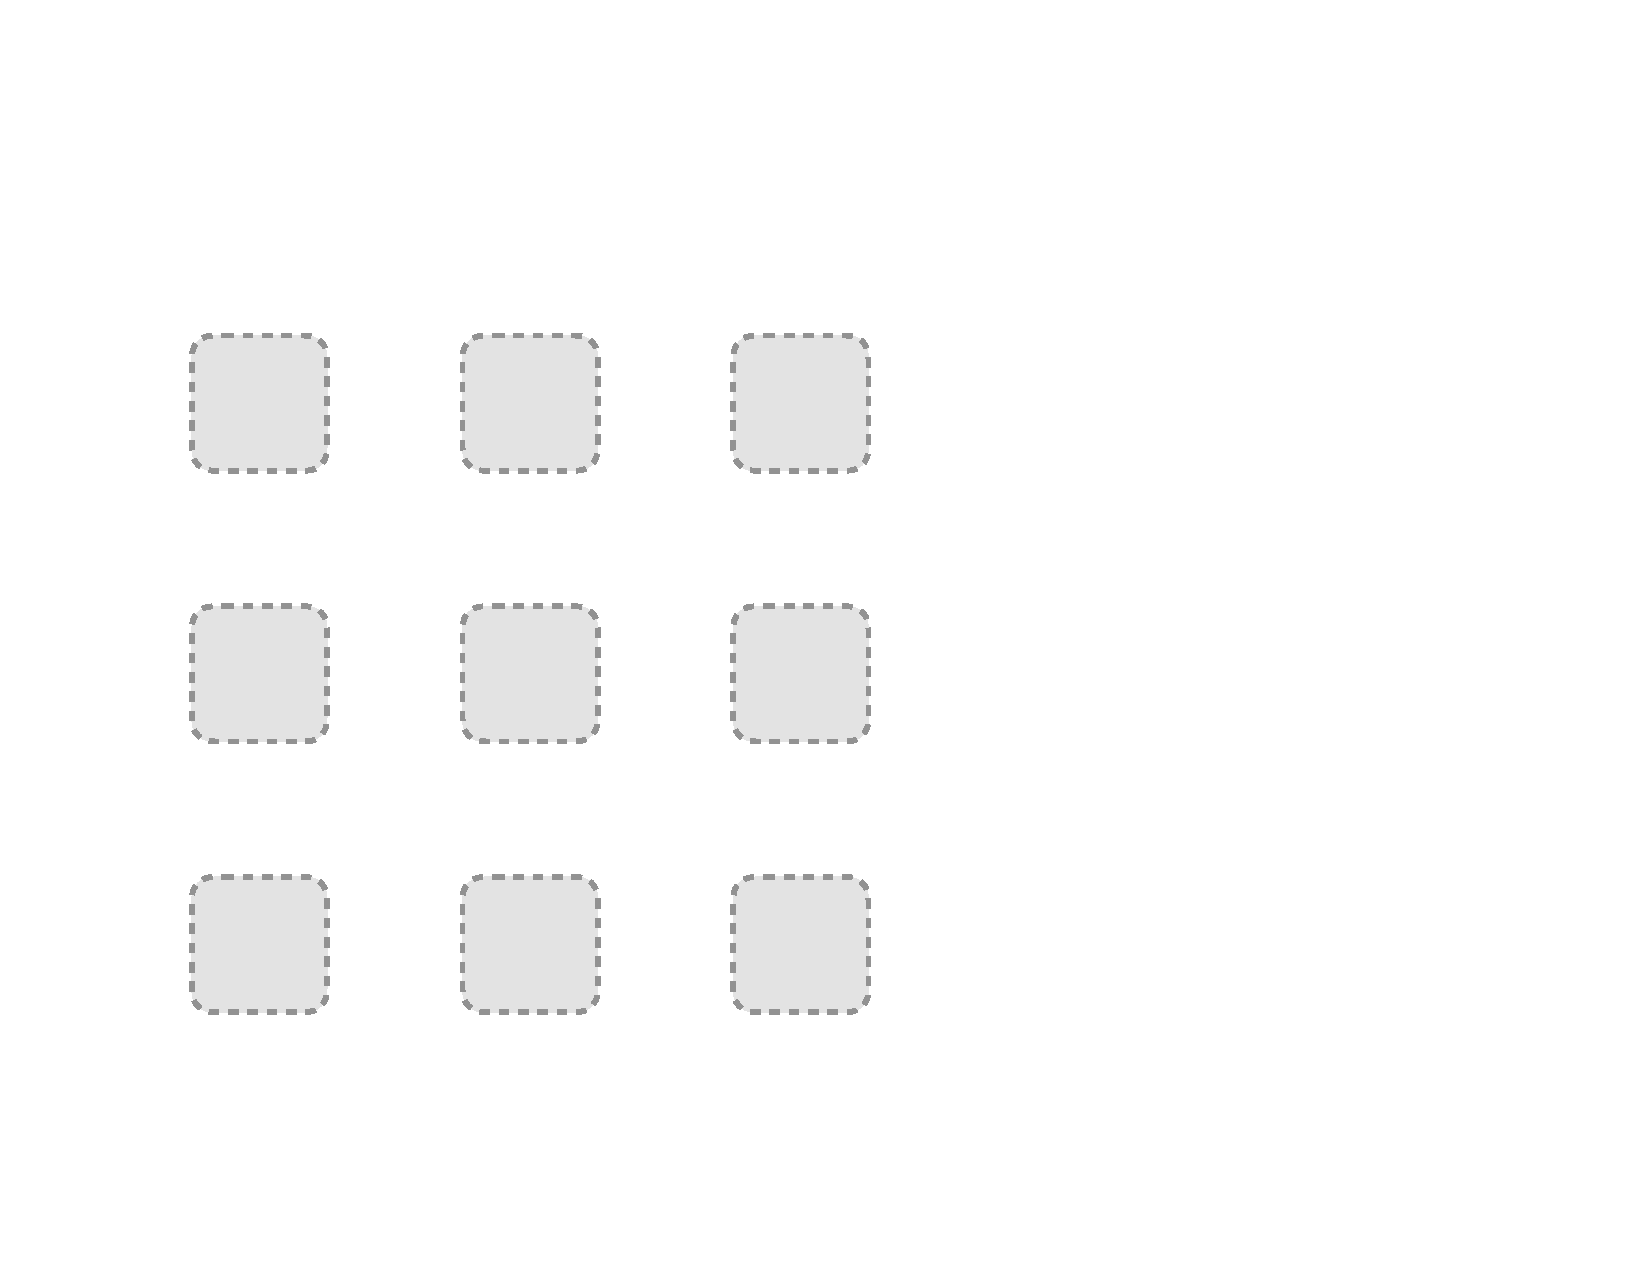
\includegraphics[draft=false,height=0.17\textheight]{figures/fig_planar}\quad\quad\quad
(b)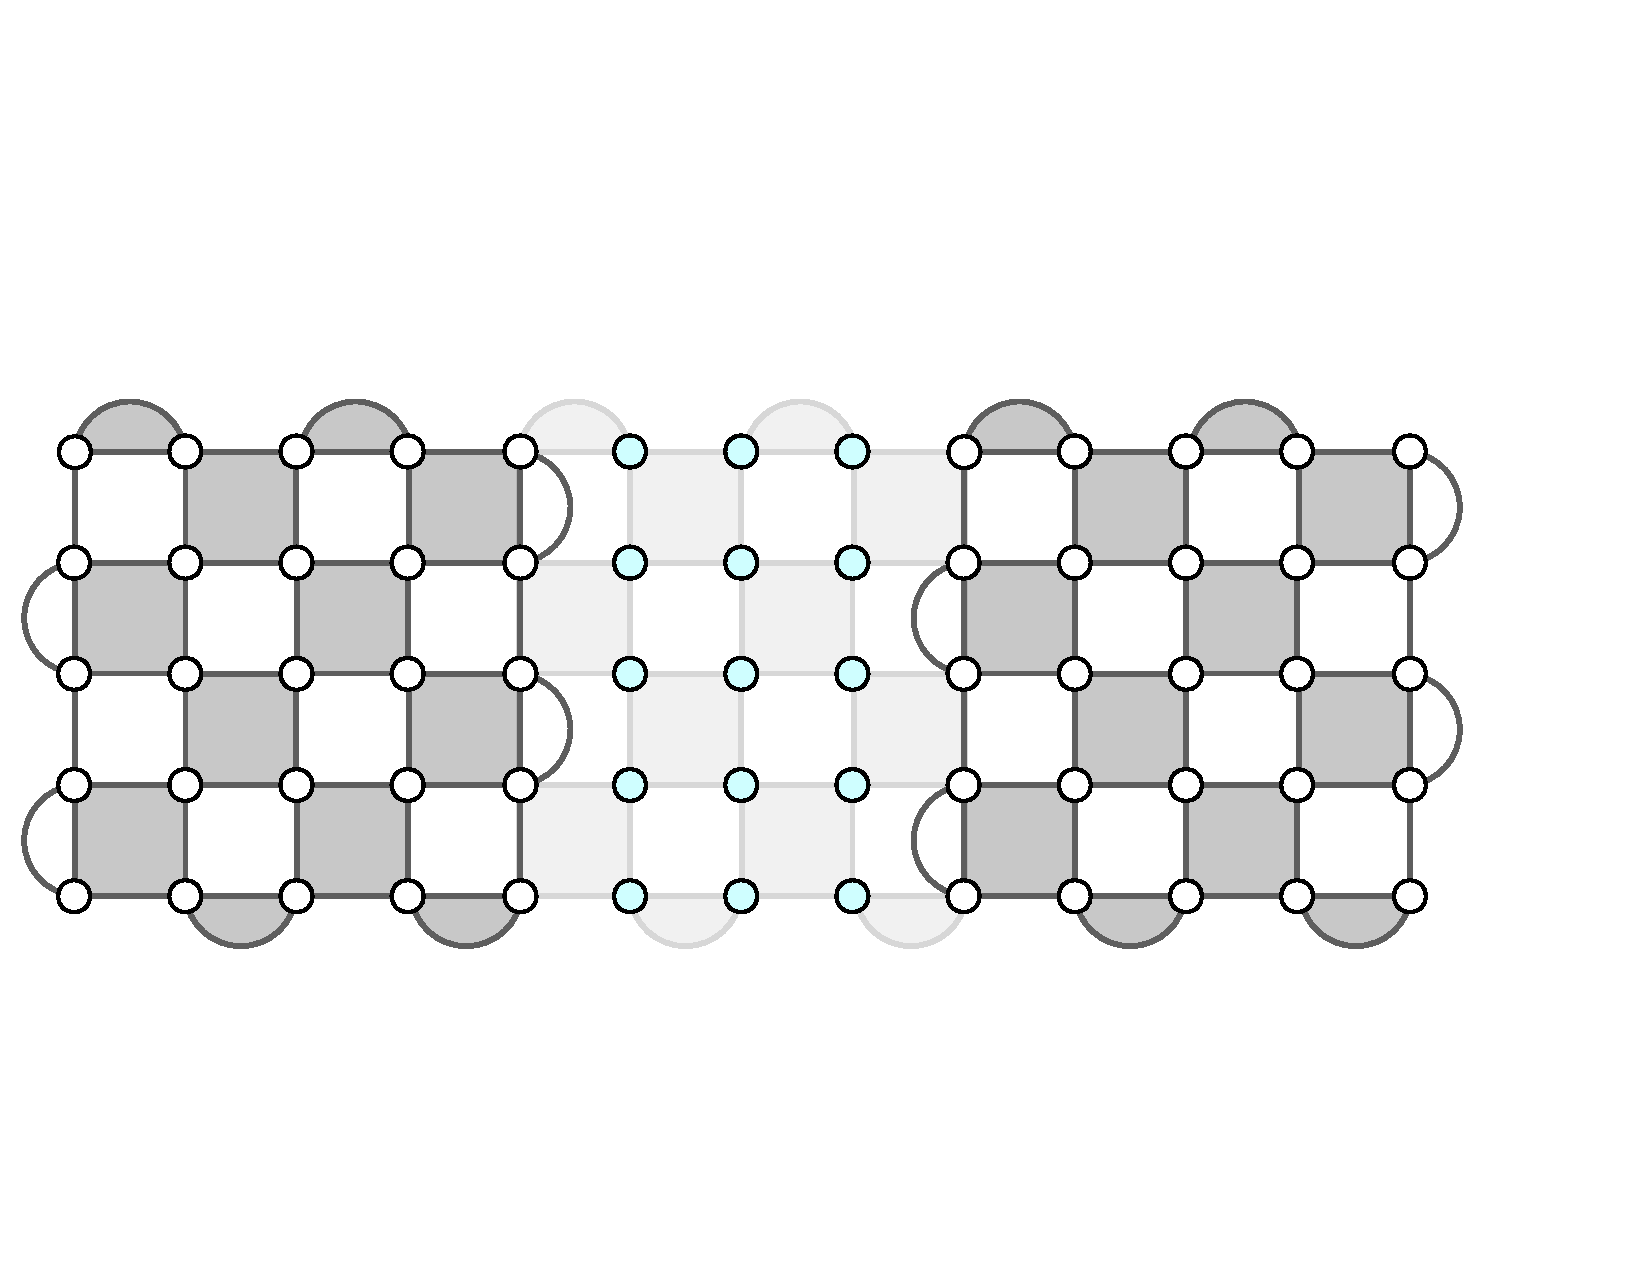
\includegraphics[draft=false,height=0.17\textheight]{figures/fig_surgery}
\caption{
(a) A planar layout of qubits comprises surface code patches (shaded), each using the layout depicted in~\cref{fig:surface_code}(a) and encoding a logical qubit, and the routing space in between. 
(b) Logical Pauli measurement $\overline{M_{XX}}$ is implemented by preparing the routing space qubits (turquoise dots) in the state $\ket 0$ and repeatedly measuring parity checks (lightly shaded) in the routing space spanning between the two surface code patches.
Other logical Pauli measurements, e.g., $\overline{M_{ZZ}}$ and $\overline{M_{YZ}}$, require connecting different boundaries of the two patches.
}
\label{fig:planar}
\end{figure}


%%%%%%%%%%%%%%%%%%%%%%%%%%%%%%%%%%%%%%%%%%%%%%%%%%%%%%%%%%%%%%%%%%%%%%

\subsubsection*{Rough overview (in math)}


The logical $\overline H$ does not pose any challenges.
From a practical standpoint, it is transversal, since it can be realized by applying the Hadamard gate $H$ to every data qubit in the surface code patch, followed by swapping of the roles of Pauli $Z$- and $X$-type parity checks in the subsequent QEC rounds.
As such, the logical $\overline H$ takes constant time and the surface code patch is effectively rotated (which may alter how subsequent operations are implemented).


The logical $\overline{CX}$ is more challenging than the logical $\overline H$, since it is impossible to implement it transversally with the planar layout of qubits and nearest-neighbor entangling gates shown in~\cref{fig:planar}(a).
Instead, one can use the following quantum circuit, where the first qubit (top wire) is the control and the third qubit (bottom wire) is the target of the logical $\overline{CX}$ gate
\begin{equation}
\begin{split}
\Qcircuit @C=.7em @R=.3em {
	& \ustick{a} \cwx[1]		& 					& 				&		\\	
	& \multigate{1}{\overline{M_{ZZ}}} 	& \qw 				& \gate{\overline{Z}^{\, b}}		& \qw		\\
\lstick{\ket{\overline{+}}}& \ghost{M_{ZZ}} 		& \multigate{1}{\overline{M_{XX}}} 	& \gate{\overline{M_Z}}		& \rstick{c}\cw	\\
	& \qw 				& \ghost{M_{XX}} 		& \gate{\overline{X}^{\, a+c}}	& \qw 		\\
	& 					& \dstick{b} \cwx[-1]		& 				&
}\\
\ 
\end{split}
\end{equation}
It is straightforward to fault-tolerantly realize preparation of the logical state $\ket{\overline{+}}$, logical Pauli measurement $\overline{M_Z}$, and logical Pauli operators $\overline{Z}$ and $\overline{X}$.
In addition, the required logical Pauli measurements $\overline{M_{ZZ}}$ and $\overline{M_{XX}}$ can be implemented fault-tolerantly via ``lattice surgery'' techniques~\cite{horsman2012latticeSurgery}; see~\cref{fig:planar}(b) for an illustration of how to realize $\overline{M_{XX}}$.
Unlike the logical $\overline H$, logical Pauli measurements $\overline{M_{ZZ}}$ and $\overline{M_{XX}}$ and, subsequently, the logical $\overline{CX}$ cannot be realized in constant time; rather, due to the need to account for measurement errors, they typically incur time overhead of $\bigO{d}$.


The logical $\overline T$ can be implemented using gate teleportation~\cite{gottesman1999viabilityUniversalQC} via the following quantum circuit
\begin{equation}
\begin{split}
\Qcircuit @C=.7em @R=.3em {
					& \multigate{1}{\overline{CX}}	& \gate{\overline{S}^{\, a}} & \qw		\\
\lstick{\ket{\overline{T}}} 	& \ghost{\overline{CX}}		& \gate{\overline{M_Z}}	& \rstick{a} \cw 
}
\end{split}
\label{eq:gate_teleportation}
\end{equation}
where the logical resource state $\ket{\overline{T}} = \left(\ket{\overline{0}} + e^{i\pi/4}\ket{\overline{1}}\right)/\sqrt{2}$, the logical gate $\overline{S} = \overline{Z}^{\,1/2}$, and the first qubit (top wire) is the control and the second qubit (bottom wire) is the target of the logical $\overline{CX}$ gate.
Even though the logical $\overline{S}$ is a Clifford gate, its fault-tolerant implementation with the surface code may not be effortless~\cite{brown2017pokingHoles} (unless one uses nonlocal entangling gates~\cite{kubica2015unfoldingColorCode,moussa2016transversalCliffordGates})
Moreover, the need to apply the logical $\overline{S}$ conditioned on the measurement outcome of $\overline{M_Z}$ may slow down quantum computation.
For that reason, it may be beneficial to use the following quantum circuit from \cite[Fig.~17(b)]{litinski2019gameofsurfacecodes}
\begin{equation}
\begin{split}
\Qcircuit @C=.7em @R=.3em {
			& \ustick{a} \cwx[1]		& 							& 					&			\\	
\lstick{\ket{\overline{0}}}& \multigate{1}{\overline{M_{YZ}}} 	& \gate{\overline{H}^{\, b}}	& \gate{\overline{M_Z}}	& \rstick{c}\cw	\\
\lstick{\ket{\overline{T}}}& \ghost{M_{YZ}} 		& \multigate{1}{\overline{M_{ZZ}}} 	& \gate{\overline{M_X}}	& \rstick{d}\cw	\\
			& \qw 				& \ghost{M_{ZZ}} 				& \gate{\overline{Z}^{\, ab+c+d}}& \qw 		\\
			& 					& \dstick{b} \cwx[-1]				& 					&
}\\
\ 
\end{split}
\label{eq:autocorrected}
\end{equation}
which is an alternative to the one in~\cref{eq:gate_teleportation} that uses one additional logical qubit but requires only logical Pauli corrections, rather than logical Clifford corrections.
In either case, given the logical resource state $\ket{\overline T}$, the logical $\overline T$ typically incurs time overhead of $\bigO{d}$.
We conclude that implementing the logical $\overline T$ reduces to the problem of preparing the logical state $\ket{\overline{T}}$, which, in turn, can be realized via state distillation~\cite{knill2004FTPostSelectedQC,bravyi2005UniversalQC}; see  \cite{beverland2021costUniversality} for a brief overview of state distillation.


%%%%%%%%%%%%%%%%%%%%%%%%%%%%%%%%%%%%%%%%%%%%%%%%%%%%%%%%%%%%%%%%%%%%%%

\subsubsection*{Dominant resource cost (gates/qubits)}


State distillation provides a fault-tolerant method to prepare high-fidelity logical resource states, such as the logical state $\ket{\overline T}$.
The basic idea is to convert some number of noisy resource states into fewer but, crucially, less noisy resource states.
Importantly, this task can be accomplished with quantum circuits comprising only Clifford gates (together with state preparation and measurement in the computational basis) and postselection.
Typically, state distillation circuits are based on some QEC code, e.g., the 15-qubit Reed--Muller code.

State distillation is often described as a resource-intensive method that contributes the most to the resource overhead of fault-tolerant quantum computation with the surface code~\cite{fowler2012SurfaceCodes} and, for that reason, many efforts have been devoted to finding possible alternatives~\cite{bravyi2015doubledColorCodes,jochymOConnor2016stackedCodes,bombin20182DquantumComputation,chamberland2019faultTolerantMagicStateFlagQubits,beverland2021costUniversality}. 
However, recent results indicate that state distillation may not be as costly as one may think~\cite{litinski2019gameofsurfacecodes,litinski2019magicstate}, especially when one optimizes it for specific quantum hardware and noise that exhibits some bias~\cite{litinski2022activeVolume}.
In the task of estimating the ground state energy density of the \hyperref[appl:FermiHubbard]{Fermi--Hubbard model}, state distillation of logical Toffoli resource states injected one at a time uses less than $10\%$ of the total resources and is never a bottleneck on runtime of the quantum algorithm~\cite{chamberland2022buildingFTQC}.


Oftentimes, a quantum algorithm is expressed as a quantum circuit $\mathcal C$ comprising Clifford and $T$ gates.
Thus, by using the aforementioned logical gates $\overline H$, $\overline{CX}$, and $\overline{T}$, we can fault-tolerantly implement the logical quantum circuit $\overline{\mathcal C}$ with the surface code of code distance $d$ and a planar layout of qubits in~\cref{fig:planar}(a).
However, from the perspective of reducing the resource overheads, it may be beneficial  to consider a quantum circuit $\mathcal C'$ equivalent to the circuit $\mathcal C$, which is obtained from $\mathcal C$ by commuting all Clifford gates to the end of $\mathcal C$~\cite{litinski2019gameofsurfacecodes}.
As a result, the circuit $\mathcal C'$ only comprises multiqubit Pauli $\pi/8$ rotations (which are a generalization of the $T$ gate and can be realized via, e.g., quantum circuits analogous to the one in~\cref{eq:autocorrected}).
Consequently, fault-tolerant implementation of the logical circuit $\overline{\mathcal{C}'}$ incurs the qubit overhead of $\bigO{Nd^2}$ and time overhead of $\bigO{Md}$, where $N$ and $M$ are the number of, respectively, qubits and $T$ gates in $\mathcal C$.
We remark that the time overhead can be reduced at the expense of increased qubit overhead---first by distilling more resource states and being able to use them faster, then by implementing them in parallel~\cite{litinski2019gameofsurfacecodes}.


%%%%%%%%%%%%%%%%%%%%%%%%%%%%%%%%%%%%%%%%%%%%%%%%%%%%%%%%%%%%%%%%%%%%%%

\subsubsection*{Caveats}


Lattice surgery is not necessary to realize fault-tolerant quantum computation with a planar layout of qubits and nearest-neighbor gates.
An alternative approach (which actually preceded the development of lattice surgery) relies on the surface code with defects and braiding~\cite{raussendorf2007FTQChighThreshold,raussendorf2007topologicalFaultTolerance,fowler2012SurfaceCodes,brown2017pokingHoles}.
However, resource overhead estimates strongly suggest that this approach is not competitive with lattice surgery~\cite{fowler2018}.


A simple architecture depicted in~\cref{fig:planar}(a) can be improved in a couple ways to reduce the qubit overhead.
First, it is possible to pack surface code patches more densely, resulting in more logical qubits for the given total number of qubits and target code distance~\cite{lao2018mappingLatticeSurgery,litinski2019gameofsurfacecodes}
Second, one can designate certain regions, commonly referred to as magic state factories, to solely produce resource states, such as the logical state $\ket{\overline T}$, and optimize their design~\cite{OGorman2017magicStateFactories,litinski2019gameofsurfacecodes,litinski2019magicstate}.


To simplify implementation of logical gates, one can consider other QEC codes, e.g., the three-dimensional color code~\cite{bombin2015gaugeColorCodes,kubica2015universalTransversalGates}.
The gauge color code has redundant degrees of freedom, commonly referred to as gauge qubits. 
For different states of its gauge qubits, the gauge color code admits transversal implementation of different logical gates, which, \emph{combined}, form a universal gate set (thus circumventing the Eastin--Knill theorem~\cite{eastin2009RestrictionsTransversal,zeng2011Transversality}).
Importantly, changing the state of gauge qubits can be done fault-tolerantly in constant time.
However, to realize this construction one needs, for instance, a three-dimensional layout of qubits with nearest-neighbor gates or a planar layout of qubits with a limited number of nonlocal gates, which are more challenging to engineer compared to the simple architecture in~\cref{fig:planar}(a).
To achieve code distance $d$ with the gauge color code one incurs qubit overhead of $\bigO{d^3}$ (compared to qubit overhead of $\bigO{d^2}$ for the surface code), so, similarly to single-shot QEC described in~\cref{prim:QEC}, this approach trades time overhead for qubit overhead. 


%%%%%%%%%%%%%%%%%%%%%%%%%%%%%%%%%%%%%%%%%%%%%%%%%%%%%%%%%%%%%%%%%%%%%%

\subsubsection*{Example use cases}


\begin{itemize}
\item Lattice surgery techniques developed for the surface code can be straightforwardly adapted to, e.g., the color code~\cite{landahl2014colorCodeLatticeSurgery} or the surface code with a twist~\cite{yoder2017surfaceCodeTwist}, leading to fault-tolerant quantum computation with potentially reduced qubit overhead.
In addition, lattice surgery techniques can also be used for the fault-tolerant transfer of encoded information between arbitrary topological quantum codes~\cite{poulsenNautrup2017faultTolerantInterface}.
\item 
Now, we are ready to present a rough, order-of-magnitude estimate of the resource overheads needed to realize fault-tolerant quantum computation in the architecture based on the surface code and lattice surgery.
For concreteness, we consider the circuit noise of strength $p=0.001$, where each basic operation, including state preparation, CNOT gate, and measurement, can fail with probability $p$.
Assume that we want to implement a quantum circuit $\mathcal C$ comprising $N=10^3$ qubits and a certain number $M=10^{10}$ of $T$ gates. These resource counts are in the ballpark of estimates for various quantum algorithms in the application areas of \hyperref[appl:QuantumChemistry]{quantum chemistry}, hyperref[appl:CondensedMatter]{condensed matter physics}, and \hyperref[appl:cryptanalysis]{cryptanalysis}.
First, following the procedure from~\cite{litinski2019gameofsurfacecodes}, we compile $\mathcal C$ into a new circuit $\mathcal C'$ of depth $M$ that comprises $N$ qubits and $M$ multiqubit Pauli $\pi/8$-rotations implemented one at a time.
Since there are $NM$ possible fault locations in the circuit $\mathcal C'$, the error rate for each qubit of $\mathcal C'$ should not exceed than
\begin{equation}
\epsilon \approx 1/(N M).
\end{equation}
Since each qubit of $\mathcal C'$ is realized as a logical qubit of the surface code with distance $d$, then its
logical error rate $p_\text{fail}$ can be approximated by 
\begin{equation}
p_\text{fail} \approx \alpha (p/p_\text{th})^{d/2},
\end{equation}
where we can crudely set $\alpha = 0.05$ and $p_\text{th} = 0.01$; see \hyperref[prim:QEC]{quantum error correction with the surface code} for more details.
Note that these values are empirical and depend heavily on the choice of the decoder; in our case---the belief-matching algorithm~\cite{higgott2023improvedDecodingCircuitNoise}.
Thus, in order for the logical error rate $p_\text{fail}$ to reach the target error rate $\epsilon$ we need the surface code distance at least
\begin{equation}
d \approx \left\lceil 2 \log(\alpha N M)/\log(p_\mathrm{th}/p) \right\rceil.
\end{equation}
Assuming that half of all required qubits is devoted to realizing $N$ surface code patches (each comprising $2d^2-1$ data and ancilla qubits), with the other half used for resource state distillation and routing,
we obtain that the fault-tolerant implementation of $\mathcal C'$ incurs qubit overhead of
\begin{equation}
n_{\mathcal C'} \approx 4Nd^2
\end{equation}
and time overhead of
\begin{equation}
t_{\mathcal C'} \approx Md\tau,
\end{equation}
where we crudely set $\tau = 1\ \!\mu s$ to be the time needed to implement one syndrome measurement round with the superconducting circuits architecture.
Finally, our order-of-magnitude resource estimate gives $2.3\times 10^6$ physical qubits and $67$ hours of runtime.
This general approach to resource estimation has been applied to a number of specific quantum algorithms in a variety of \hyperref[applications]{application areas}; see, e.g.,~\cite{lee2021EvenMoreEfficientChemistryTensorHyp, gidney2021HowToFactor, Kivlichan2020ImprovedFaultTolerantSimulationCondensedMatter,Beverland2022Requirements,sanders2020FTQCforCombOpt}. These references often go beyond a back-of-the-envelope calculation and provide a more meticulous analysis that accounts for exact qubit layouts and the physical footprint of resource state distillation factories. They also pursue optimizations to how the circuit is implemented (e.g.~exploiting space-time tradeoffs) in light of these considerations. 

\end{itemize}



%%%%%%%%%%%%%%%%%%%%%%%%%%%%%%%%%%%%%%%%%%%%%%%%%%%%%%%%%%%%%%%%%%%%%%

\subsubsection*{Further reading}

\begin{itemize}
\item An accessible overview of fault-tolerant quantum computation based on the surface code and lattice surgery can be found in  \cite{litinski2019gameofsurfacecodes}. 
\item A convenient way to describe and optimize lattice surgery operations is via the ZX calculus, which is a diagrammatic language for quantum computing~\cite{coecke2017picturingQuantumProcesses,deBeaudrap2020ZXcalculusLatticeSurgery}.
\item A direct comparison of the resource overhead associated with preparation of the logical resource state $\ket{\overline T}$ using either state distillation or transversal gates (with the three-dimensional color code) can be found in  \cite{beverland2021costUniversality}.
\item To read about a framework for estimating resources required to realize large-scale fault-tolerant quantum computation, see  \cite{Beverland2022Requirements}.
\end{itemize}

%%%%%%%%%%%%%%%%%%%%%%%%%%%%%%%%%%%%%%%%%%%%%%%%%%%%%%%%%%%%%%%%%%%%%%
\printbibliography[heading=secbib,segment=\therefsegment]

\end{refsection}